\documentclass[12pt,a4paper,titlepage]{article}
\usepackage[utf8]{inputenc}
\usepackage[finnish]{babel}
\usepackage{setspace}
\usepackage{subcaption}
\usepackage{fancyhdr}
\usepackage[top=1in, bottom=1in, left=1in, right=1in]{geometry}
\usepackage{float}
\usepackage{pdfpages}
\usepackage{enumitem}

\usepackage{hyperref}
\hypersetup{pdfborder={0 0 0}}
\onehalfspacing
\cfoot{}
\rhead{\thepage}
\lhead{\leftmark}

\title{Tsoha\\ Kurssikysely \vspace{0.5em}}
\author{Anni Järvenpää}
\date{\today}

\begin{document}
\maketitle

% Sisällysluettelo
\newpage
\tableofcontents
\thispagestyle{empty}
\newpage
\setcounter{page}{1}
\parskip=1em \advance\parskip by 0pt plus 2pt
\pagestyle{fancy}
\cfoot{\thepage}

%%%%%%%%%%%%%%% Oleellinen sisältö alkaa%%%%%%%%%%%%%%%
\section{Johdanto}
Työn tavoitteena on toteuttaa kurssikyselyjärjestelmä, jonka avulla opiskelijoilta voidaan kerätä palautetta kursseista. Järjestelmää voidaan käyttää koko tiedekunnassa ja kyselyt sisältävätkin sekä koko tiedekunnan laajuisia kysymyksiä että laitos- ja kurssikohtaisia kysymyksiä. Kysymysten vastaukset voivat olla avoimia tai ne voidaan valita numeroasteikolta tai muusta annetusta arvojoukosta.

Kurssin luennoitsija voi lisätä, poistaa ja muokata kurssikohtaisia kysymyksiä ja laitoksen ja tiedekunnan hallintohenkilöstö niiden kysymyksiä. Samoin uusille kursseille voidaan luoda uusia kyselyitä ja vanhoja voidaan poistaa. Kyselyn muokkaaminen tai poistaminen edellyttää kuitenkin, ettei kysely ole parhaillaan käynnissä.

Laitos ja tiedekunta voivat hakea yhteenvedon kurssin tai kurssien kysymysten tuloksista kuten vastaajamääristä tai tiettyyn kysymykseen saaduista vastauksista. Kurssin pitäjä saa järjestelmästä yksityiskohtaisen raportin kyselyn tuloksista aina halutessaan.


\section{Yleiskuva järjestelmästä}
Järjestelmää käyttävät opiskelijat, opettajat ja laitoksen sekä tiedekunnan hallintohenkilöt. Näistä kaikki voivat kirjautua järjestelmään ja tarkastella kyselyitä. Näkyvät kyselyt ja niille tehtävissä olevat operaatiot riippuvat kuitenkin käyttäjäryhmästä. Käyttö\-tapaus\-kaavio on nähtävillä kuvassa \ref{fig:kayttotapauskaavio}.

\begin{figure}
   \centering
   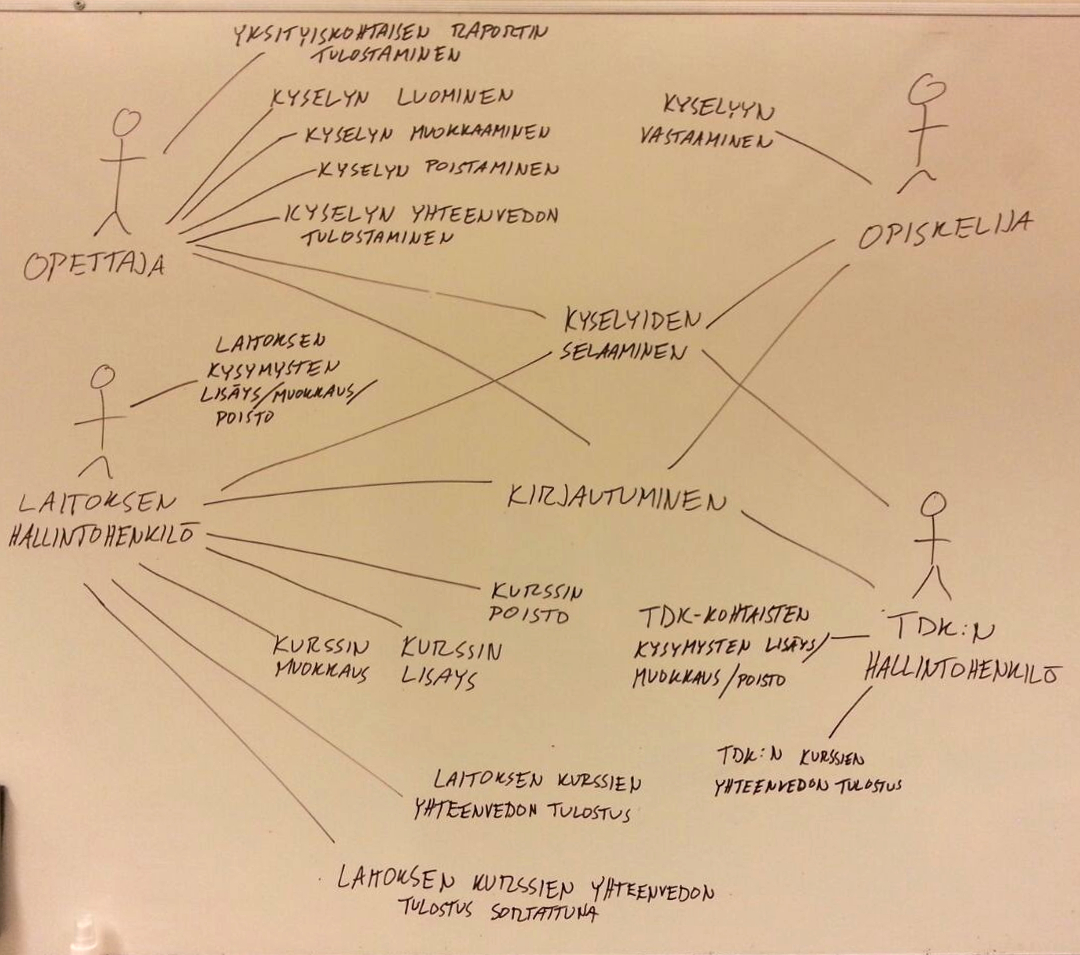
\includegraphics[width=\textwidth]{kuvat/kayttotapauskaavio.jpg}
   \caption{Järjestelmän käyttötapauskaavio}\label{fig:kayttotapauskaavio}
\end{figure}

Jokaisen käyttäjäryhmän käyttäjät voivat kirjautua palveluun ja selata kyselyitä. Käyttäjälle näytettävä valikoima kuitenkin vaihtelee: opiskelija näkee ainoastaan avoimet kyselyt niiltä kursseilta, joilla on osallistujana, opettaja ainoastaan omien kurssiensa kyselyt ja laitoksen hallintohenkilöt ainoastaan oman laitoksen kurssit. Tiedekunnan hallintohenkilöt puolestaan näkevät kaikkien kurssien kyselyt. Kyselyihin pystyy vastaamaan ainoastaan opiskelija.

Tiedekuntakohtaisten kysymysten luomisesta sekä tarvittaessa muokkaamisesta ja poistamisesta vastaa tiedekunnan hallintohenkilö. Tätä varten kysymykset on toki voitava myös listata, vaikka sitä ei ole piirretty näkyviin käyttötapauskaavioon. Lisäksi tiedekunnan hallintohenkilö voi tulostaa nähtävilleen yhteenvedon kyselyiden tuloksista.

Laitoksen hallintohenkilöt vastaavat laitoskohtaisten kysymysten luomisesta, muokkaamisesta ja poistamisesta. Heidän tehtävänään on pitää esimerkiksi kurssin vastuuopettajatiedot ajantasaisina. Lisäksi he luovat uudet kurssit ja hoitavat muuttuneiden kurssitietojen muokkaamisen tai valikoimasta poistuneiden kurssien poistamisen. Vastaavasti kuin tiedekuntakohtaisissa kysymyksissä, laitoksen hallintohenkilöt voivat tarkastella laitoskohtaisiin kysymyksiin saatujen vastausten yhteenvetoja.

Kurssin opettaja voi lisätä omille kursseilleen kyselyitä. Niitä voi myös muokata tai poistaa, ei kuitenkaan silloin, kun ne ovat avoimina eli opiskelijat voivat vastana niihin. Myös opettaja voi pyytää yhteenvetoraportin jonkin kyselyn tuloksista. Koska esimerkiksi tekstimuotoisten kysymysten tapauksessa on yksittäisten vastausten tarkasteleminen tarpeen, voidaan myös yksittäisen kurssin kyselyn kaikki vastaukset näyttää yksityiskohtaisessa raportissa.

Yhteenvetoraporttia tulostettaessa laitoksen ja tiedekunnan hallintohenkilöt näkevät aina omalle organisaatiotasolleen spesifien kysymysten vastausten keskiarvot ja -hajonnat sekä vastaajamäärät. Näkymä voidaan haluttaessa järjestää tietyn kysymyksen vastausten perusteella. Tästä syystä tiedekunta- tai laitoskohtaisten kysymysten vastaukset voivat olla ainoastaan numeerisia.

Vastaavasti opettaja voi tulostaa yhteenvetoraportin tietyn kyselyn vastauksista, jolloin hän saa nähtäväkseen kustakin kyselyn kysymyksestä vastauksien keskiarvon ja keskihajonnan. Opettaja voi halutessaan tarkastella myös yksityiskohtaisia raportteja kursseistaan, jolloin hän saa nähtäväkseen kyselyn kunkin kysymyksen vastausjakauman (monivalintakysymykset) tai kaikki annetut vastaukset (aviomet kysymykset).

\section{Järjestelmän tietosisältö}

\section{Relaatiotietokantakaavio}

\section{Järjestelmän yleisrakenne}

\section{Käyttöliittymä ja järjestelmän komponentit}

\section{Asennustiedot}

\section{Käynnistys- ja käyttöohje}



%%%%% Sisältö loppuu, lähdeluettelo %%%%%
\bibliographystyle{plain}
\small
\bibliography{lahteet}

\appendix
%\newpage
\section{Tärkeä liite}
Lorem ipsum.
\newpage



\end{document}
